\documentclass[a4paper, 12pt]{book}
% preamble.tex

\usepackage[utf8]{inputenc}
\usepackage[T1]{fontenc}
\usepackage[english]{babel} % Ho cambiato in italian, supponendo che la maggior parte del testo sia in italiano
\usepackage{amsmath}
\usepackage{amssymb}
\usepackage{graphicx}
\usepackage{hyperref}
\usepackage{geometry}
\usepackage{fontspec} % Utile per Xetex/LuaLaTeX ma mantenuto
\usepackage{booktabs}
\usepackage{amsthm}
\usepackage{enumitem}
\usepackage{caption}
\usepackage{thmtools}
\usepackage{standalone} % Già presente nel tuo elenco
\usepackage{tkz-euclide}
\usepackage{graphicx}
\usepackage[T1]{fontenc}
\usepackage{wesa}

% --- PACCHETTI AGGIUNTI PER LA FORMATTAZIONE ---
\usepackage{parskip}  % Aggiunge spazio tra i paragrafi (stile "blocco")
\usepackage{fancyhdr} % Per intestazioni e piè di pagina personalizzati

% --- IMPOSTAZIONI GEOMETRIA E FONT ---
\geometry{a4paper, margin=1in}

% Configura lo stile 'plain' (usato da \maketitle e \tableofcontents)
% per essere coerente con il piè di pagina
\fancypagestyle{plain}{
    \fancyhf{} % Pulisce
    \cfoot{\thepage} % Mette solo il numero di pagina
    \renewcommand{\headrulewidth}{0pt} % Niente linea su queste pagine
}

% Configurazione Header/Footer per le altre pagine
\pagestyle{fancy}
\fancyhead{} % Pulisce l'intestazione
\fancyfoot{} % Pulisce il piè di pagina
\fancyhead[L]{\nouppercase{\rightmark}} % Nome Sezione a sinistra (o Chapter)
\fancyhead[R]{\nouppercase{\leftmark}}  % Nome Capitolo a destra (o Sezione)
\fancyfoot[C]{\thepage} % Numero di pagina al centro
\renewcommand{\headrulewidth}{0.4pt}
\renewcommand{\footrulewidth}{0pt}


% --- DEFINIZIONI TEOREMI ---
% (Questa parte è cruciale per la tua struttura)
\newtheoremstyle{mythmstyle}%
    {}%
    {}%
    {\itshape}%
    {}%
    {\bfseries}%
    {}%
    { }%
    {\thmname{#1}\thmnumber{ #2}%
    \thmnote{: #3\addcontentsline{toc}{subsubsection}{{\itshape#1}: #3}}. }

% 2. Imposta questo stile come quello ATTUALE
\theoremstyle{mythmstyle}

\newtheorem{theorem}{Th}[section]
\newtheorem{definition}{Def}[section]
\newtheorem{proposition}{Prop}[section]
\newtheorem{corollary}{Cor}[section]
\newtheorem{algorithm}{Alg}[section]
\newtheorem{lemma}{Lemma}[section]
\newtheorem*{remark}{Rem}

% Definizioni utili per il Main file
\newcommand{\inputlesson}[1]{\clearpage\input{#1}\clearpage} % Comando per input lezione
\usepackage[x11names]{xcolor}
\usepackage{tikz}
\usetikzlibrary{shapes,fit}
\usepackage{amsmath} % Required for align environment


\begin{document}
\setcounter{chapter}{5}
\chapter{Digression on Circular Convolution}
\section{Circular Convolution}

\begin{itemize}
    \item \textbf{Problem}: in the time domain, \textbf{linear convolution} is complicated to perform.
\end{itemize}

\begin{align}
    y[n] = (x * h)[n] = \underbrace{\sum_{l=0}^{L} h[l]x[n-l]}_{\text{discrete time}}
\end{align}

Where:
\begin{itemize}
    \item $h$ is a \textbf{filter}
    \item $x$ is the \textbf{input signal}
    \item $y$ is the \textbf{output signal}
\end{itemize}

In the frequency domain, convolution becomes a simple \textbf{multiplication}!

\begin{align}
    y[n] = x[n] * h[n] \xrightarrow{\text{FFT}} Y[k] = X[k] \cdot H[k]
\end{align}

So the idea is:
\begin{enumerate}
    \item Transform the signal (f domain)
    \item Equalize it (do stuff)
    \item Transform it back (time domain)
\end{enumerate}

% Riquadro rosso "Attenzione"
\begin{tcolorbox}[colframe=red, colback=white, title=\textbf{\faExclamationTriangle \ Attention}]
    \textbf{Multiplication} holds only for \textbf{circular convolution}, not linear.
\end{tcolorbox}

We need a way to ``\textbf{trick}'' the linear convolution channel so that its output corresponds to that of a circular convolution $\implies$ \textbf{CYCLIC PREFIX (CP)}!

Suppose we have a \textbf{payload} of length $K$ and a response of the filter $h$ with \textbf{memory} or order $L$.

The \textbf{CP} is obtained by taking the last $L_{cp}$ samples of the \textbf{payload} and \textbf{prepending} them to the start of that block.
\section{Cyclic Prefix \& Fourier Taxonomy}

To guarantee that the \textbf{linear convolution} is equal to the \textbf{circular} one, we must have $L_{cp} \ge L$.

\begin{figure}[h]
    \centering
    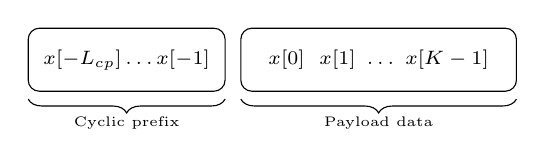
\begin{tikzpicture}
        % Nodes for the boxes
        \node[draw, rounded corners, minimum width=2.5cm, minimum height=0.8cm] (cp) at (0,0) {\scriptsize $x[-L_{cp}] \dots x[-1]$};
        \node[draw, rounded corners, minimum width=3.5cm, minimum height=0.8cm] (payload) at (3.2,0) {\scriptsize $x[0] \ \ x[1] \ \dots \ x[K-1]$};
        
        % Braces under the boxes
        \draw[decorate, decoration={brace, amplitude=5pt, mirror}] (-1.25,-0.5) -- (1.25,-0.5) node[midway, below=3pt] {\tiny Cyclic prefix};
        \draw[decorate, decoration={brace, amplitude=5pt, mirror}] (1.45,-0.5) -- (4.95,-0.5) node[midway, below=3pt] {\tiny Payload data};
    \end{tikzpicture}
\end{figure}

I obtain an \textbf{extended signal} $\overline{x}[n]$ of length $K + L_{cp}$.
In this way, the \textbf{periodic input} necessary for the \textbf{circular convolution} is simulated.

\vspace{1em}

% Tabella/Albero di classificazione Time/Fourier
\begin{center}
\renewcommand{\arraystretch}{2}
\begin{tabular}{c | l}
    \textbf{\textcolor{cyan}{TIME DOMAIN}} & \textbf{\textcolor{cyan}{FOURIER}} \quad {\scriptsize F.T. exists} \\
    \hline
    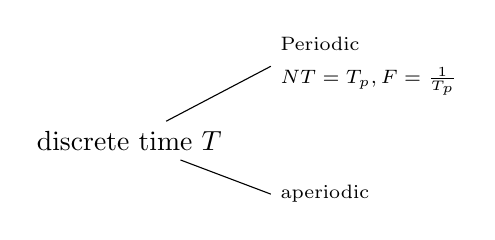
\begin{tikzpicture}[baseline=(current bounding box.center)]
        \node (root) {discrete time $T$};
        \node (per) [above right=0.2cm and 0.5cm of root, align=left] {\scriptsize Periodic \\ \scriptsize $NT=T_p, F=\frac{1}{T_p}$};
        \node (aper) [below right=0.2cm and 0.5cm of root] {\scriptsize aperiodic};
        \draw (root) -- (per.west);
        \draw (root) -- (aper.west);
    \end{tikzpicture} 
    & 
    \begin{minipage}{6cm}
        $S(kF) = \sum_{n=0}^{N-1} s(nT) e^{-j 2\pi k F n T}$ \\
        $S(f) = \sum_{n=-\infty}^{+\infty} s(nT) e^{-j 2\pi f n T}$
    \end{minipage} 
    \\
    \hline
    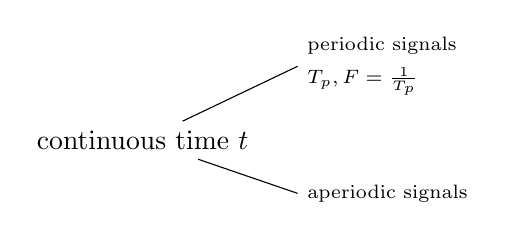
\begin{tikzpicture}[baseline=(current bounding box.center)]
        \node (root) {continuous time $t$};
        \node (per) [above right=0.2cm and 0.5cm of root, align=left] {\scriptsize periodic signals \\ \scriptsize $T_p, F=\frac{1}{T_p}$};
        \node (aper) [below right=0.2cm and 0.5cm of root] {\scriptsize aperiodic signals};
        \draw (root) -- (per.west);
        \draw (root) -- (aper.west);
    \end{tikzpicture}
    & 
    \begin{minipage}{6cm}
        $S(kF) = \int_{0}^{T_p} s(t) e^{-j 2\pi k t} dt$ \\
        $S(f) = \int_{-\infty}^{+\infty} s(t) e^{-j 2\pi f t} dt$ \\
        {\scriptsize $\uparrow$ this is a generic case}
    \end{minipage}
\end{tabular}
\end{center}

We focus on the behavior at \textbf{discrete periodic time}.

\begin{minipage}{0.45\textwidth}
    \textbf{discrete time periodic}:
    \begin{align}
        \sum s(n) e^{-j 2\pi \frac{kn}{N}}
    \end{align}
    $\rightarrow$ Also called \textbf{Discrete Fourier Transform (DFT)}.
\end{minipage}
\hfill
\begin{minipage}{0.45\textwidth}
    \centering
    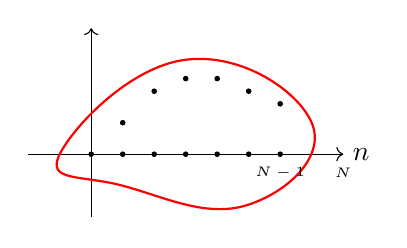
\begin{tikzpicture}[scale=0.8]
        \draw[->] (-1,0) -- (4,0) node[right] {$n$};
        \draw[->] (0,-1) -- (0,2);
        
        % Samples
        \foreach \x in {0,0.5,...,3}
            \filldraw (\x, 0) circle (1pt);
            
        \foreach \x/\y in {0.5/0.5, 1/1, 1.5/1.2, 2/1.2, 2.5/1, 3/0.8}
            \filldraw (\x, \y) circle (1pt);

        % Red envelope shape
        \draw[red, thick] plot [smooth cycle, tension=0.8] coordinates {(-0.5,0) (1.5,1.5) (3.5,0.5) (2.5,-0.8) (0.5,-0.5)};
        
        \node at (3, -0.3) {\tiny $N-1$};
        \node at (4, -0.3) {\tiny $N$};
    \end{tikzpicture}
\end{minipage}

\vspace{1em}

The \textbf{circular convolution} is defined as:
\begin{align}
    c(n) = \sum_{l=0}^{K-1} h[l] x[(n-l)_N]
\end{align}

Relationship in frequency domain:
\begin{align}
    \textcolor{cyan}{C(k)} = \textcolor{cyan}{H(k)} \cdot \textcolor{cyan}{X(k)}
\end{align}

\section{Graphical Representation: SC-FDE}

\begin{figure}[h]
    \centering
    
\includegraphics[width=0.9\textwidth]{Pictures/image.png}
    \caption{SC-FDE}
    \label{fig:SC-FDE}
\end{figure}

\subsection{Receiver Structure Notes}

\begin{itemize}
    \item \textbf{Simple transmitter}, complicated receiver.
    \item We can put the equalizer in the transmitter to make it more balanced.
\end{itemize}

% --- PLACEHOLDERS FOR FIGURES ---
\begin{figure}[h]
    \centering
    
\includegraphics[width=0.6\textwidth]{Pictures/image copy.png}
    \caption*{Fig. 2.14 Top: Serial-to-parallel, DFT, Equalization, IDFT}
    \label{fig:SC-FDE}
\end{figure}
    
    \vspace{1cm}

    \begin{figure}[h]
    \centering
    
\includegraphics[width=0.6\textwidth]{Pictures/image copy 2.png}
    \caption*{Fig. 2.14 Bottom: Channel taps into DFT}
    \label{fig:SC-FDE}
    \end{figure}

% --------------------------------

\subsection{Noise Variance Derivation}

\begin{align}
    &= \frac{N_0}{G} U^* \text{diag}\left( \frac{1}{|h[0]|} \dots \frac{1}{|h[K-1]|} \right) \text{diag}\left( \frac{1}{h[0]} \dots \frac{1}{h[K-1]} \right)^* U \tag{2.197} \\
    &= \frac{N_0}{G} U^* \text{diag}\left( \frac{1}{|h[0]|^2}, \dots, \frac{1}{|h[K-1]|^2} \right) U. \tag{2.198}
\end{align}

The above covariance matrix is, in general, not proportional to the identity, indicating that the noise is correlated. The \textbf{variance of the noise} on the $n$-th equalized symbol is:

\begin{align}
    &\left[ \frac{N_0}{G} U^* \text{diag}\left( \frac{1}{|h[0]|^2}, \dots, \frac{1}{|h[K-1]|^2} \right) U \right]_{n,n} \tag{2.199} \\
    &= \frac{N_0}{G K} \sum_{k=0}^{K-1} e^{-j\frac{2\pi}{K}nk} \frac{1}{|h[k]|^2} e^{j\frac{2\pi}{K}nk} \tag{2.200} \\
    &= \frac{N_0}{G K} \sum_{k=0}^{K-1} \frac{1}{|h[k]|^2} \tag{2.201}
\end{align}

which does not depend on $n$, revealing that the noise variance is constant over the output.

\end{document}